\documentclass[lettersize,journal]{IEEEtran}
\usepackage{amsmath,amsfonts}
\usepackage{algorithmic}
\usepackage{algorithm}
\usepackage{array}
\usepackage[caption=false,font=normalsize,labelfont=sf,textfont=sf]{subfig}
\usepackage{textcomp}
\usepackage{stfloats}
\usepackage{url}
\usepackage{verbatim}
\usepackage{graphicx}
\usepackage{cite}
\usepackage{xspace}
\usepackage{multirow}
\usepackage[hidelinks]{hyperref}
\usepackage{balance}
\usepackage{amsmath}
\usepackage{amssymb}
\usepackage{booktabs}
\hyphenation{op-tical net-works semi-conduc-tor IEEE-Xplore}
% updated with editorial comments 8/9/2021

\newtheorem{definition}{Definition}[section]
\newtheorem{theorem}{Theorem}[section]
\newtheorem{lemma}{Lemma}
\newtheorem{proof}{Proof}[section]

%\SetAlFnt{\scriptsize}	
%\SetAlCapFnt{\scriptsize}
%\SetAlCapNameFnt{\scriptsize}
%\SetFuncSty{textsf}

%\tikzset{help lines/.style={color=gray!30,very thin}}
\newcommand\subtitle[1]{{\large #1}} 
\newcommand{\superscript}[1]{\ensuremath{^{\textrm{#1}}}}
\newcommand{\Rmnum}[1]{\uppercase\expandafter{\romannumeral #1}}  %定义命令输入大写罗马数字
\newcommand{\rmnum}[1]{\romannumeral #1}  
%定义命令输入小写罗马数字

\usepackage{adjustbox}

\def\tu{\superscript{\dag}}
\def\gu{\superscript{\ddag}}
\def\tulab{\superscript{\S}}
\def\nulab{\superscript{\P}}


\renewcommand{\algorithmicrequire}{ \textbf{Input:}} %Use Input in the format of Algorithm
\renewcommand{\algorithmicensure}{ \textbf{Output:}} %UseOutput in the format of Algorithm

\newcommand{\ragname}{CoverRAG\xspace}

\begin{document}

% \title{CoverRAG: Claim-Oriented Verification and Evidence-Routed Retrieval-Augmented Generation}
\title{CoverRAG: Coverage-Guided Claim Verification for Plug-and-Play Retrieval-Augmented Generation}

\author{Jiake Ge,
        Hui Wang,
        Xin Wang,~\IEEEmembership{Member,~IEEE,}
        Yunpeng Chai,~\IEEEmembership{Member,~IEEE}
        

\IEEEcompsocitemizethanks{\IEEEcompsocthanksitem 
Jiake Ge is with the School of Artificial Intelligence, Tianjin University, Tianjin 300354, China. E-mail: gejiake@tju.edu.cn.
Hui Wang is with the School of Computer Software, Tianjin University, Tianjin 300354, China. E-mail: haileywang@tju.edu.cn.
Yunpeng Chai is with the School of Information, Renmin University of China, Beijing 100872, China. E-mail: ypchai@ruc.edu.cn.
Xin Wang is with the School of Artificial Intelligence, Tianjin University, Tianjin 300354, China. E-mail: wangx@tju.edu.cn.
}

% <-this % stops an unwanted space
}

% The paper headers
\markboth{Journal of \LaTeX\ Class Files,~Vol.~14, No.~8, August~2024}%
{Shell \MakeLowercase{\textit{et al.}}: A Sample Article Using IEEEtran.cls for IEEE Journals}

\maketitle

\begin{abstract}
Retrieval-augmented generation (RAG) improves language models by grounding answers in external evidence, yet retrieved documents that are relevant to a question do not necessarily support every factual claim in the generated answer. This gap is especially problematic for long-form and attributed generation, where an answer may contain many atomic claims, only some of which are actually covered by the cited evidence. We propose \textsc{CoverRAG}, a plug-and-play controller that treats RAG as a claim-level evidence coverage problem. Given a draft answer from any RAG backbone, \textsc{CoverRAG} decomposes it into atomic claims, verifies each claim against evidence, constructs a coverage state over supported and unresolved answer units, plans missing answer-unit targets, retrieves or selects evidence only for those targets, and accepts new content only when it both fills a missing answer unit and is supported by evidence. The final answer is generated from the supported coverage state under citation and output-quality guards. Experiments on ASQA, ELI5, and QAMPARI with vanilla RAG, Self-RAG, and BGE-rerank RAG show that \textsc{CoverRAG} consistently improves claim support and citation faithfulness while preserving or improving main task performance. On the strongest BGE-rerank backbone, \textsc{CoverRAG} improves average main correctness by 0.78 points, sentence-level citation recall by 3.88 points, claim citation recall by 54.07 points, and claim citation precision by 29.26 points.
\end{abstract}

\begin{IEEEkeywords}
Retrieval-augmented generation, attributed generation, factuality verification, citation faithfulness, claim verification, plug-and-play RAG.
\end{IEEEkeywords}


\section{Introduction}
\label{sec:introduction}

Retrieval-augmented generation (RAG) has become a standard paradigm for grounding large language models in external knowledge sources~\cite{lewis2020retrieval,gao2023retrieval}. A RAG system retrieves documents or passages for a user question and conditions a generator on the retrieved context. This interface makes RAG attractive for knowledge-intensive question answering, enterprise assistants, scientific search, and attributed generation, where users expect answers to be both useful and inspectable.

However, document relevance is not the same as answer support. A retrieved passage can be relevant to the question but fail to support a particular factual statement in the generated answer. A citation can support one fact in a sentence while leaving another fact unsupported. A generator can also combine retrieved content with unsupported parametric knowledge. These failures are common in long-form and attributed generation, where a single answer may contain many atomic factual claims with different evidence needs~\cite{gao2023enabling,wallat2025correctness}.

The key limitation is that many RAG systems are controlled at the level of queries, documents, passages, or whole responses, while faithfulness failures occur at the level of individual answer claims. Consider a question that asks for several attributes of an entity. A retriever may find evidence for some attributes but not others. The generator may nevertheless produce a complete-looking answer by filling the missing attribute from parametric knowledge or by copying a weakly related passage. A sentence-level citation checker may observe that the sentence has a citation, but this does not imply that every atomic claim in the sentence is entailed by the cited source.

We argue that reliable RAG requires an explicit \emph{claim-level evidence coverage} state: which answer units are already supported, which claims are unsupported, which claims lack citations, which citations point to the wrong evidence, and which answer units remain missing. This state should not only be used for post-hoc evaluation. It should control how the system spends additional retrieval, verification, and generation budget.

We propose \textsc{CoverRAG}, a coverage-guided claim verification controller for plug-and-play RAG. Given a draft answer from any RAG backbone, \textsc{CoverRAG} decomposes the answer into atomic claims, verifies each claim against evidence, and builds a coverage state over supported and unresolved answer units. Supported claims form an intermediate supported answer. Unsupported, uncited, or wrongly cited claims reveal possible coverage gaps. The controller then plans concrete missing answer-unit targets, retrieves or selects evidence only for those targets, and accepts a new claim only if it both fills a missing answer unit and is supported by evidence.

\begin{figure}[t]
    \centering
    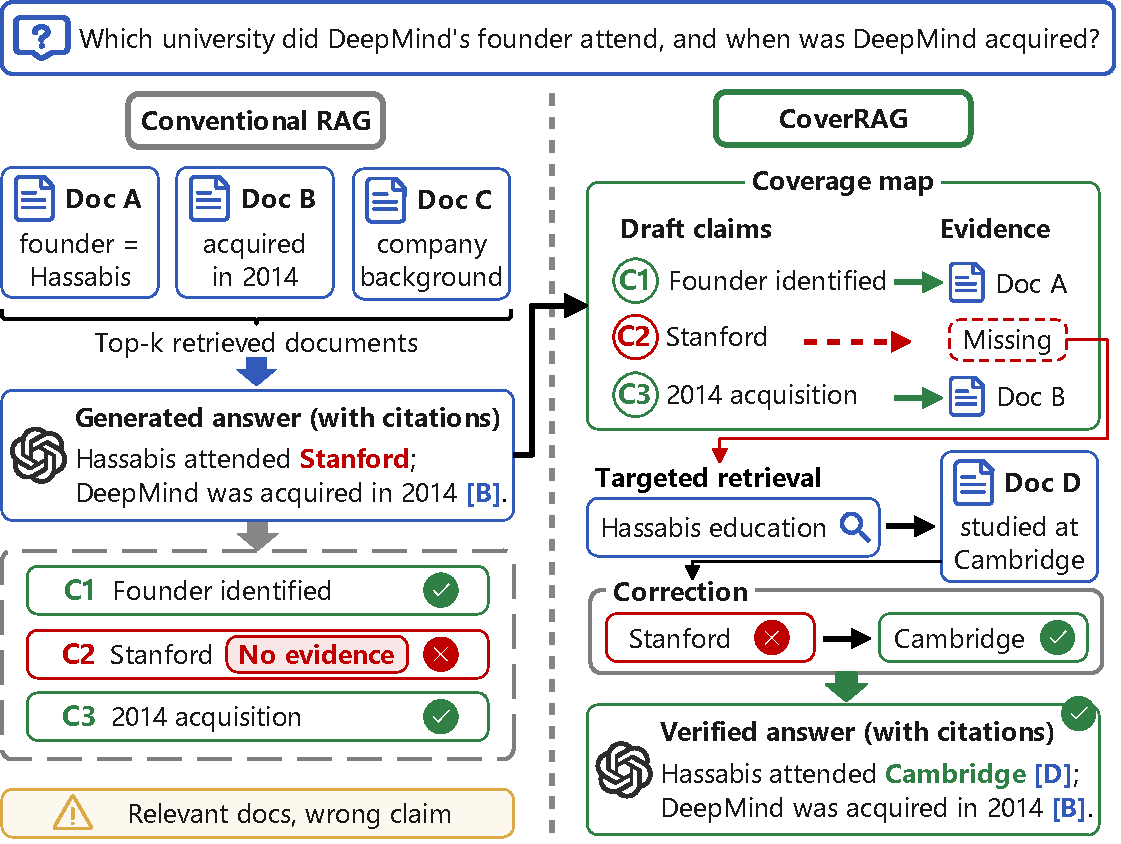
\includegraphics[width=\linewidth]{figs_wh/bg.pdf}
    \caption{Conventional RAG optimizes retrieved context for the original query. \textsc{CoverRAG} instead maintains a claim-level coverage state and uses unresolved answer units to guide retrieval, verification, and guarded answer update.}
    \label{fig:motivation}
\end{figure}

\autoref{fig:motivation} illustrates the distinction. Standard RAG produces an answer from an initial evidence pool. \textsc{CoverRAG} treats that answer as a hypothesis to be audited. The controller asks: which claims are supported, which answer units remain missing, and which new claims can be safely added without degrading citation faithfulness? Retrieval is then targeted by the original question, the missing answer unit, optional evidence clues, and the already supported answer state. This discourages redundant search for already covered content and focuses the evidence budget on unresolved answer units.

The design is plug-and-play. \textsc{CoverRAG} does not require modifying the internals of the base retriever or generator. It only assumes access to a draft answer and a candidate evidence pool. We instantiate it on three backbones: vanilla RAG, Self-RAG~\cite{asai2024self}, and BGE-rerank RAG. These backbones differ in how they generate the draft answer; \textsc{CoverRAG} adds the same answer-side coverage controller after generation.

Our evaluation uses ASQA, ELI5, and QAMPARI from the attributed long-form generation setting~\cite{gao2023enabling}. We report task correctness and task recall, sentence-level citation recall and precision, claim-level citation recall and precision, claim sentence recall, and claim support. This evaluation is necessary because a system can improve citation precision by deleting information, or improve support by adding facts that are supported but irrelevant. \textsc{CoverRAG} is designed to improve claim support and citation faithfulness while preserving useful answer content.

This paper makes the following contributions:

\begin{itemize}
    \item We formulate RAG answer refinement as \emph{claim-level evidence coverage}, explicitly tracking supported, unsupported, uncited, and wrongly cited atomic answer claims.
    \item We introduce \textsc{CoverRAG}, a coverage-guided iterative controller that plans missing answer-unit targets, retrieves or selects evidence for those targets, and accepts new content only when it is both coverage-improving and evidence-supported.
    \item We demonstrate plug-and-play effectiveness across vanilla RAG, Self-RAG, and BGE-rerank RAG on three attributed generation datasets, showing large gains in claim support and citation faithfulness while preserving or improving main task performance.
\end{itemize}

Overall, \textsc{CoverRAG} advances a simple view: trustworthy RAG should not only retrieve relevant documents, but should optimize the coverage relation between answer claims and supporting evidence.


\section{Related Work}
\label{sec:related_work}

\subsection{Retrieval-Augmented Generation}

RAG grounds language models in non-parametric evidence and has been advanced through dense retrieval, sparse retrieval, reranking, retrieval-augmented pretraining, and multi-passage generation~\cite{guu2020retrieval,lewis2020retrieval,karpukhin2020dense,izacard2021leveraging,izacard2023atlas,borgeaud2022improving,robertson2009probabilistic,nogueira2019passage}. These methods improve the chance that useful evidence appears in the context window. However, they mostly optimize retrieval relevance or context quality. They do not guarantee that every factual claim in the final answer is supported by the evidence that is retrieved or cited.

\subsection{Adaptive and Corrective RAG}

Adaptive and self-corrective RAG methods decide when to retrieve, critique evidence, revise generations, or interleave retrieval with reasoning~\cite{asai2024self,yan2024corrective,jeong2024adaptive,shao2023enhancing,trivedi2023interleaving,yao2023react}. These systems move beyond one-shot retrieve-then-generate pipelines. Their control signals, however, are commonly defined over retrieval actions, passage utility, generated responses, or reasoning states. \textsc{CoverRAG} is complementary: it defines the control state over atomic answer claims and their evidence coverage.

\subsection{Attributed Generation and Citation Evaluation}

Attributed generation aims to make generated answers verifiable by linking them to sources~\cite{bohnet2022attributed,gao2023enabling,gao2023rarr}. Prior work shows that citations should be evaluated rather than treated as surface markers of reliability. Yet sentence-level citation evaluation can miss mixed-support sentences, where one cited source supports only part of a sentence. \textsc{CoverRAG} moves attribution to the claim level: each atomic claim is verified against evidence, and citation assignment is constrained by claim support.

\subsection{Factuality Verification and Claim Decomposition}

Fact verification and factuality evaluation provide tools for detecting unsupported content~\cite{thorne2018fever,min2023factscore,manakul2023selfcheckgpt,dhuliawala2024chain}. These methods often decompose generations into checkable facts or ask verification questions. \textsc{CoverRAG} uses such tools as part of an inference-time controller: verification results are not only scores, but actions that determine whether to preserve, repair, retrieve for, or suppress a claim.

\subsection{Knowledge- and Graph-Enhanced RAG}

Recent graph- and knowledge-enhanced RAG systems organize external evidence with graph structures, entity relations, or multimodal sources~\cite{edge2024local,guo2024lightrag,wang2024knowledge,zhao2024kg,chen2022murag}. These approaches improve evidence access and reasoning structure. \textsc{CoverRAG} is orthogonal to the evidence backend: its abstraction is the coverage relation between answer claims and evidence units. The same controller can be layered above text retrievers, rerankers, document graphs, or knowledge-graph retrieval systems.


\section{Problem Formulation}
\label{sec:problem_formulation}

Let $q$ be a user question and let $\mathcal{E}=\{e_1,\ldots,e_N\}$ be a collection of retrievable evidence units. A base RAG system retrieves an initial evidence pool $\mathcal{E}_0 \subseteq \mathcal{E}$ and generates a draft answer $\tilde{a}$. The goal of \textsc{CoverRAG} is to transform $\tilde{a}$ into a final answer $a$ whose answer-bearing claims are covered by verifiable evidence.

\subsection{Atomic Claims and Evidence Labels}

We decompose an answer into atomic factual claims:
\begin{equation}
    \mathcal{C}(a)=\{c_1,\ldots,c_m\}.
\end{equation}
An atomic claim is a minimal factual statement that can be independently checked against evidence. For each claim $c_i$, a verifier examines a candidate evidence set $S_i \subseteq \mathcal{E}$ and returns a label
\begin{equation}
    z_i = V(c_i,S_i) \in \mathcal{Y}.
\end{equation}
In our implementation, $\mathcal{Y}$ contains four operational states:
\begin{equation}
    \mathcal{Y}=\{\mathsf{SUP},\mathsf{UNSUP},\mathsf{NOCITE},\mathsf{BADCITE}\}.
\end{equation}
$\mathsf{SUP}$ means the claim is supported by evidence. $\mathsf{UNSUP}$ means available evidence does not support it. $\mathsf{NOCITE}$ means the answer presents the claim without a usable citation. $\mathsf{BADCITE}$ means the attached citation is missing or points to evidence that does not entail the claim.

\subsection{Claim-Level Coverage State}

At iteration $t$, \textsc{CoverRAG} maintains a coverage state
\begin{equation}
    \mathcal{M}^{t}=(\mathcal{C}^{t},\mathcal{S}^{t},\mathcal{Z}^{t},\Gamma^{t},\mathbf{r}^{t}),
\end{equation}
where $\mathcal{C}^{t}$ is the current claim set, $\mathcal{S}^{t}$ stores claim-specific evidence, $\mathcal{Z}^{t}$ stores verification labels, $\Gamma^{t}$ stores citation links, and $\mathbf{r}^{t}$ stores confidence scores. The supported coverage state is
\begin{equation}
    \mathcal{C}^{+,t}=\{c_i^t:z_i^t=\mathsf{SUP}\}.
\end{equation}
This set is used as a compact representation of what the answer already covers reliably.

\subsection{Missing Answer-Unit Targets}

We define a missing answer-unit target as a concrete answer span or claim fragment that is likely useful for answering $q$ but is not covered by $\mathcal{C}^{+,t}$. Targets are generated from two sources: unsupported or citation-broken draft claims, and high-ranked evidence sentences that contain plausible answer spans not already covered by supported claims. A target is discarded if it is already covered, duplicated, generic, title-like, or irrelevant to the question.

\subsection{Objective}

The controller should improve answer utility while respecting a bounded budget of retrieval, verification, and generation calls. Conceptually, it optimizes
\begin{align}
    \max_{\pi}\quad
    &\mathrm{Correct}(a,q)
    +\lambda_1\mathrm{Recall}(a,q)
    +\lambda_2\mathrm{ClaimSupport}(a,\mathcal{E}) \nonumber\\
    &+\lambda_3\mathrm{CitationFaith}(a,\Gamma)
    -\lambda_4\mathrm{Unsupported}(a,\mathcal{E})
    -\lambda_5\mathrm{Cost}(\pi).
\end{align}
This objective is not used as a differentiable training loss. Instead, \textsc{CoverRAG} approximates it with a rule-based and verifier-guided controller that only adds content when it is both answer-useful and evidence-supported.


\section{The \textsc{CoverRAG} Framework}
\label{sec:framework}

\textsc{CoverRAG} is a plug-in controller placed after a base RAG generator. It takes a question, a draft answer, and an evidence pool as input, then iteratively updates a claim-level coverage state. The loop is shown in Algorithm~\ref{alg:coverrag}.

\begin{algorithm}[t]
\caption{\textsc{CoverRAG}: Coverage-Guided Claim Controller}
\label{alg:coverrag}
\begin{algorithmic}[1]
\REQUIRE question $q$, draft answer $\tilde{a}$, evidence pool $\mathcal{E}_0$, retriever or evidence provider $R$, verifier $V$, budget $B$
\ENSURE final answer $a$ with claim-level citations
\STATE decompose $\tilde{a}$ into atomic claims $\mathcal{C}^{0}$
\STATE initialize evidence sets and coverage state $\mathcal{M}^{0}$
\FOR{$t=0,1,\ldots$ while budget remains}
    \STATE verify each unresolved or newly added claim in $\mathcal{M}^{t}$
    \STATE construct supported state $\mathcal{C}^{+,t}$
    \STATE generate missing answer-unit targets $\mathcal{T}^{t}$
    \IF{$\mathcal{T}^{t}$ is empty}
        \STATE break
    \ENDIF
    \STATE retrieve or rerank evidence for targets in $\mathcal{T}^{t}$
    \STATE generate candidate answer-unit claims from new evidence
    \STATE filter candidates with answer-unit and output guards
    \STATE verify remaining candidates with $V$
    \STATE add supported candidates to $\mathcal{M}^{t+1}$
\ENDFOR
\STATE render final answer from supported claims and citations
\STATE audit final answer and remove unsupported residual claims
\STATE \textbf{return} $a$
\end{algorithmic}
\end{algorithm}

\subsection{Draft Audit and Claim Verification}

The base RAG system first produces a draft answer. \textsc{CoverRAG} decomposes the draft into atomic claims and verifies them against their cited evidence or the available evidence pool. Verification produces four operational labels: supported, unsupported, no citation, and wrong or missing citation. These labels are stored in the coverage state and determine subsequent actions. Supported claims are preserved. Unsupported or citation-broken claims become possible sources of missing targets. Background claims are down-weighted so that the controller does not waste retrieval budget on low-value details.

\subsection{Supported Answer State}

The supported claims are summarized into an intermediate supported answer state. This state is not a final response. It is a memory of already covered answer units. It plays two roles. First, it prevents the system from retrieving repeatedly for content that is already supported. Second, it gives the generator and retriever a compact context for deciding what remains missing.

\subsection{Missing Target Planning}

The controller builds missing answer-unit targets from two sources. The first source is rejected draft claims: if a draft claim is unsupported, uncited, or wrongly cited, its protected answer spans and salient phrases are treated as candidate missing targets. The second source is evidence: high-ranked evidence sentences may contain answer spans not yet covered by supported claims. These spans are treated as hypothesized missing answer units.

Not every target is retained. The planner removes targets that are already covered by supported claims, duplicated under normalized span keys, too generic, title-like, source-fragment-like, or unrelated to the question. The result is a small set of concrete targets such as an entity, date, number, causal mechanism, condition, or explanatory phrase.

\subsection{Coverage-Guided Retrieval}

For each retained target, \textsc{CoverRAG} constructs a retrieval query that combines the original question, the missing answer unit, optional evidence clues, and a brief supported-answer summary:
\begin{equation}
    \bar{q}=\operatorname{Query}(q,\mathrm{target},\mathrm{clue},\mathcal{C}^{+}).
\end{equation}
This differs from ordinary query expansion. The query explicitly represents what is already answered and what remains missing. The retriever or candidate evidence provider then returns additional evidence for these target-specific queries.

\subsection{Answer-Unit Gate}

New evidence can contain many supported but irrelevant facts. Therefore, a candidate claim is not accepted merely because it is entailed by evidence. It must first pass an answer-unit gate. The candidate must match a missing target through normalized answer-span keys or lexical overlap, must be relevant to the original question, must expose a concrete answer span, and must avoid generic or title-like surfaces.

We score a candidate by
\begin{equation}
\begin{split}
    s_{\mathrm{unit}} =
    &0.35s_{\mathrm{target}}
    +0.25s_{\mathrm{question}}
    +0.25s_{\mathrm{span}} \\
    &+0.15s_{\mathrm{rank}}
    -p_{\mathrm{compact}},
\end{split}
\end{equation}
where $s_{\mathrm{target}}$ measures target match, $s_{\mathrm{question}}$ measures question relevance, $s_{\mathrm{span}}$ rewards explicit answer spans, $s_{\mathrm{rank}}$ uses evidence ranking, and $p_{\mathrm{compact}}$ penalizes overly long, generic, or type-mismatched candidates. Explanation questions use stricter directness checks so that isolated names or titles are not accepted as explanatory coverage.

\subsection{Evidence Verification and Guarded Update}

Only candidates that pass the answer-unit gate are verified by the evidence verifier. A candidate is added to the coverage state only if the verifier labels it as supported. The final renderer then constructs an answer from supported claims, preserving verified draft content and inserting only a small number of high-confidence new claims. A final audit decomposes the rendered answer again and removes residual unsupported claims introduced during verbalization.

The resulting loop can be summarized as:
\begin{equation}
\small
\begin{split}
&\mathrm{draft}
\rightarrow \mathrm{claim\ audit}
\rightarrow \mathrm{supported\ state}
\rightarrow \mathrm{missing\ targets}\\
&\rightarrow \mathrm{targeted\ retrieval}
\rightarrow \mathrm{answer\mbox{-}unit\ gate}
\rightarrow \mathrm{verification}
\rightarrow \mathrm{guarded\ update}.
\end{split}
\end{equation}


\section{Experiments}
\label{sec:experiments}

\subsection{Experimental Setup}

\textbf{Datasets.} We evaluate on three attributed generation datasets: ASQA, ELI5, and QAMPARI~\cite{gao2023enabling}. They cover ambiguous factoid question answering, long-form explanatory answering, and list-style answer generation.

\textbf{Backbones.} We test \textsc{CoverRAG} as a plug-in controller on three RAG backbones. Vanilla RAG uses the original retrieved top documents and a direct generator. Self-RAG uses a self-reflective generation pipeline~\cite{asai2024self}. BGE-rerank RAG reranks candidate documents with a cross-encoder reranker before generation.

\textbf{Implementation.} Unless otherwise noted, all reported plug-in results use the frozen \textsc{CoverRAG} v13 configuration. This version instantiates the claim audit, supported-state construction, answer-unit candidate gating, evidence verification, citation repair, recall-oriented completion, final audit, and output-selection guards. We use the same v13 controller across backbones.

\textbf{Metrics.} We report main task correctness and main task recall following the dataset evaluator. We also report sentence-level citation recall and precision, claim-level citation recall and precision, claim sentence recall, and claim support. Claim-level metrics are important because sentence-level citation scores can hide unsupported atomic claims inside cited sentences.

\subsection{Overall Results}

\begin{table*}[t]
    \centering
    \caption{Average v13 gains over the corresponding v0 backbone across ASQA, ELI5, and QAMPARI. Higher is better for all metrics.}
    \label{tab:avg_results}
    \scriptsize
    \setlength{\tabcolsep}{3pt}
    \begin{tabular}{lrrrrrrr}
        \toprule
        Backbone & Main Corr. & Main Rec. & Sent Cit. R & Sent Cit. P & Claim Cit. R & Claim Cit. P & Claim Support \\
        \midrule
        Vanilla RAG & +0.91 & +0.97 & +4.77 & +1.99 & +52.78 & +27.59 & +52.78 \\
        Self-RAG & +0.42 & +0.60 & +3.26 & +3.20 & +46.57 & +29.47 & +46.57 \\
        BGE-rerank RAG & +0.78 & +0.80 & +3.88 & +0.44 & +54.07 & +29.26 & +54.07 \\
        \bottomrule
    \end{tabular}
\end{table*}

\autoref{tab:avg_results} summarizes the average gains. \textsc{CoverRAG} improves main correctness and main recall on all three backbones. The gains are moderate, which is expected because the controller is conservative: it rejects candidates that are supported but do not fill a missing answer unit. The larger gains appear in evidence-faithfulness metrics. Claim citation recall improves by 46--54 points, and claim citation precision improves by 27--29 points. This confirms that the controller substantially changes the evidence alignment of generated answers, rather than only rewriting surface text.

\begin{table*}[t]
    \centering
    \caption{Detailed v0 vs. \textsc{CoverRAG} v13 results. Corr. and Rec. denote main task correctness and recall. Sent. R/P denote sentence-level citation recall/precision. Claim R/P denote claim-level citation recall/precision. Supp. denotes claim support.}
    \label{tab:main_results}
    \scriptsize
    \setlength{\tabcolsep}{2.5pt}
    \begin{tabular}{llrrrrrrrr}
        \toprule
        Backbone & Dataset & Corr. & Rec. & Sent. R & Sent. P & Claim R & Claim P & Claim Sent. R & Supp. \\
        \midrule
        Vanilla v0 & ASQA & 45.30 & 43.12 & 73.86 & 59.83 & 52.50 & 59.07 & 28.72 & 52.50 \\
        Vanilla + Cover & ASQA & 46.82 & 44.63 & 78.36 & 62.60 & 96.25 & 73.30 & 90.85 & 96.25 \\
        Vanilla v0 & ELI5 & 16.20 & 17.63 & 40.53 & 36.89 & 51.37 & 67.31 & 29.35 & 51.37 \\
        Vanilla + Cover & ELI5 & 16.07 & 18.50 & 47.56 & 37.55 & 95.91 & 68.43 & 92.22 & 95.91 \\
        Vanilla v0 & QAMPARI & 14.88 & 8.72 & 25.88 & 26.47 & 27.70 & 30.33 & 26.17 & 27.70 \\
        Vanilla + Cover & QAMPARI & 16.24 & 9.26 & 28.65 & 29.02 & 97.73 & 97.76 & 97.73 & 97.73 \\
        \midrule
        Self-RAG v0 & ASQA & 41.98 & 39.67 & 77.98 & 64.52 & 53.76 & 54.69 & 31.41 & 53.76 \\
        Self-RAG + Cover & ASQA & 43.23 & 41.08 & 81.25 & 69.36 & 94.29 & 71.91 & 87.19 & 94.29 \\
        Self-RAG v0 & ELI5 & 18.60 & 18.63 & 52.57 & 40.21 & 63.93 & 66.54 & 39.96 & 63.93 \\
        Self-RAG + Cover & ELI5 & 18.60 & 19.13 & 58.11 & 43.85 & 95.35 & 70.04 & 91.27 & 95.35 \\
        Self-RAG v0 & QAMPARI & 16.60 & 8.76 & 35.88 & 35.80 & 27.05 & 27.11 & 25.49 & 27.05 \\
        Self-RAG + Cover & QAMPARI & 16.63 & 8.64 & 36.84 & 36.90 & 94.82 & 94.79 & 94.82 & 94.82 \\
        \midrule
        BGE-rerank v0 & ASQA & 42.77 & 40.55 & 67.47 & 57.16 & 51.67 & 60.75 & 29.26 & 51.67 \\
        BGE-rerank + Cover & ASQA & 44.26 & 41.99 & 74.60 & 61.60 & 96.07 & 73.32 & 90.29 & 96.07 \\
        BGE-rerank v0 & ELI5 & 20.07 & 20.53 & 56.77 & 50.33 & 46.54 & 60.61 & 23.83 & 46.54 \\
        BGE-rerank + Cover & ELI5 & 20.20 & 21.10 & 59.79 & 45.97 & 96.40 & 68.84 & 93.06 & 96.40 \\
        BGE-rerank v0 & QAMPARI & 17.07 & 9.53 & 28.20 & 28.76 & 30.24 & 31.22 & 26.92 & 30.24 \\
        BGE-rerank + Cover & QAMPARI & 17.79 & 9.91 & 29.69 & 30.01 & 98.19 & 98.21 & 98.19 & 98.19 \\
        \bottomrule
    \end{tabular}
\end{table*}

\subsection{Analysis}

\textbf{Main task performance.} \textsc{CoverRAG} improves or preserves main task correctness on most settings. The largest gains appear on ASQA and QAMPARI, where citation-broken or unsupported answer units can be removed or repaired without substantially harming answer completeness. ELI5 is harder: its reference labels reward broad explanatory coverage, so aggressive support filtering can reduce some useful but weakly evidenced explanations. The answer-unit gate mitigates this by allowing only compact and question-relevant additions.

\textbf{Citation faithfulness.} Sentence-level citation recall improves for every backbone and dataset. Sentence precision also usually improves, with one notable trade-off on BGE-rerank ELI5. This case reflects a common tension in long-form explanatory generation: adding supported explanatory content can increase recall while introducing more citation links, some of which are judged less precise at the sentence level. Claim-level metrics show that the added content is nevertheless much better grounded.

\textbf{Claim support.} The largest and most consistent improvement is claim support. Across all backbones, \textsc{CoverRAG} moves claim support from roughly 43--48\% to roughly 95--97\% on average. This supports our central hypothesis: answer-side control should be evaluated at claim granularity, because sentence-level metrics alone understate the grounding improvement.

\textbf{Plug-in behavior.} The controller works on vanilla RAG, Self-RAG, and BGE-rerank RAG without changing their internal generation logic. This suggests that \textsc{CoverRAG} is not tied to a particular retriever. Instead, it complements retrieval-side improvements by adding answer-side coverage control.

\subsection{Ablation Study}

We conduct ablations on the vanilla RAG backbone to isolate the effect of the main controller components. \autoref{tab:ablation} reports macro-average changes over ASQA, ELI5, and QAMPARI relative to the full v13 system. We ablate targeted recovery, recall-oriented completion, evidence/claim expansion, final audit, audit-based output candidate selection, and the verifier type.

\begin{table*}[t]
    \centering
    \caption{Macro-average ablation results on vanilla RAG. Values are deltas relative to the full v13 system. Higher is better. Claim-level metrics for \textsc{NoFinalAudit} are unavailable because final-audit claim records are not produced when the audit is disabled.}
    \label{tab:ablation}
    \scriptsize
    \setlength{\tabcolsep}{3pt}
    \begin{tabular}{lrrrrrrrr}
        \toprule
        Setting & Main Corr. & Main Rec. & Sent. R & Sent. P & Claim R & Claim P & Claim Sent. R & Supp. \\
        \midrule
        Full v13 & 0.00 & 0.00 & 0.00 & 0.00 & 0.00 & 0.00 & 0.00 & 0.00 \\
        \textsc{NoRecovery} & -0.46 & -0.64 & +2.01 & +5.31 & -3.04 & +8.22 & -7.34 & -3.04 \\
        \textsc{NoRecallCompletion} & -0.11 & -0.17 & -0.99 & -1.27 & +0.31 & -0.00 & +0.99 & +0.31 \\
        \textsc{NoExpansion} & -0.47 & -0.81 & -4.08 & -5.14 & +2.12 & +0.30 & +4.56 & +2.12 \\
        \textsc{NoFinalAudit} & -0.04 & -0.07 & -0.03 & +0.02 & -- & -- & -- & -- \\
        \textsc{NoCandidateSelection} & -0.00 & -0.02 & +0.01 & -0.06 & -0.10 & -0.20 & -0.07 & -0.10 \\
        \textsc{LLMVerifier} & +0.34 & +0.17 & +4.20 & +6.62 & -6.06 & +17.93 & -9.95 & -6.06 \\
        \bottomrule
    \end{tabular}
\end{table*}

\textbf{Targeted recovery.} Removing targeted recovery lowers main correctness by 0.46 points and main recall by 0.64 points. It also reduces claim support by 3.04 points and claim sentence recall by 7.34 points. Sentence citation precision increases because the ablated system keeps fewer recovered links and claims, but this comes at the cost of lower answer utility and weaker claim-level coverage. Thus recovery is important for preserving supported answer content.

\textbf{Recall-oriented completion and expansion.} Removing recall-oriented completion alone causes smaller drops in main correctness and recall. Removing expansion more broadly has a larger effect: main correctness drops by 0.47 points, main recall by 0.81 points, and sentence citation recall/precision by 4.08/5.14 points. Claim support increases in the no-expansion setting because the output becomes more conservative. This confirms that expansion is the main utility-oriented component, while verification and recovery are the main faithfulness-oriented components.

\textbf{Final audit and output selection.} Disabling final audit has little effect on main and sentence-level metrics, but it removes final-audit claim records and is therefore not directly comparable for claim-level metrics. A cleaner ablation disables only audit-based output candidate selection while keeping final audit enabled. This has almost no effect on main correctness or recall and only slightly lowers claim-level metrics, suggesting that candidate selection is a stabilizer rather than the main source of the gains.

\textbf{Verifier sensitivity.} Replacing the NLI verifier with an LLM verifier improves main correctness and sentence-level citation scores, but lowers claim support by 6.06 points and claim sentence recall by 9.95 points. The effect is dataset-dependent: LLM verification is more permissive and can improve surface-level answer utility, while the NLI verifier is more conservative for claim-level support. We therefore use the NLI verifier as the default when prioritizing faithful claim coverage.

\subsection{Current Limitations}

The v13 implementation is conservative. It prioritizes evidence support and citation faithfulness over aggressive answer expansion, so main task gains are smaller than claim-support gains. The strongest future direction is to make the missing-answer-unit loop more retrieval-active: after each supported-state update, the controller should issue fresh retrieval queries for still-missing targets and repeat until the marginal answer-unit gain is exhausted. This is the coverage-guided iterative RAG direction discussed in the framework.

\section{Conclusion}
\label{sec:conclusion}

We introduced \textsc{CoverRAG}, a plug-and-play controller for claim-level evidence coverage in retrieval-augmented generation. The central idea is to control RAG at the level where faithfulness failures occur: atomic answer claims. \textsc{CoverRAG} audits a draft answer, builds a supported coverage state, identifies missing answer-unit targets, retrieves or selects evidence for those targets, verifies candidate additions, and renders a guarded final answer from supported claims.

Experiments on ASQA, ELI5, and QAMPARI show that this answer-side controller consistently improves citation faithfulness and claim support across vanilla RAG, Self-RAG, and BGE-rerank RAG, while preserving or improving main task performance. The results suggest that retrieval relevance and answer faithfulness should be treated as related but distinct objectives. Future work will extend the controller to deeper multi-round retrieval, graph-based evidence backends, and learned policies for allocating verification and retrieval budget.





\bibliography{reference}
\bibliographystyle{IEEEtran}




% \newpage

% \section{Biography Section}
% If you have an EPS/PDF photo (graphicx package needed), extra braces are
%  needed around the contents of the optional argument to biography to prevent
%  the LaTeX parser from getting confused when it sees the complicated
%  $\backslash${\tt{includegraphics}} command within an optional argument. (You can create
%  your own custom macro containing the $\backslash${\tt{includegraphics}} command to make things
%  simpler here.)
 
% \vspace{11pt}

% \bf{If you include a photo:}\vspace{-33pt}
% \begin{IEEEbiography}[{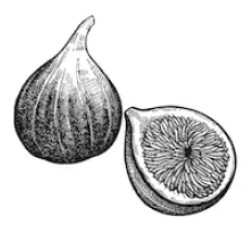
\includegraphics[width=1in,height=1.25in,clip,keepaspectratio]{fig1}}]{Michael Shell}
% Use $\backslash${\tt{begin\{IEEEbiography\}}} and then for the 1st argument use $\backslash${\tt{includegraphics}} to declare and link the author photo.
% Use the author name as the 3rd argument followed by the biography text.
% \end{IEEEbiography}

% \vspace{11pt}






% \vfill

\end{document}
